\begin{figure}
  \caption{\label{fig:intern_map} Proportion of 1940 Japanese population interned}
  \begin{adjustbox}{width=\textwidth, center}
    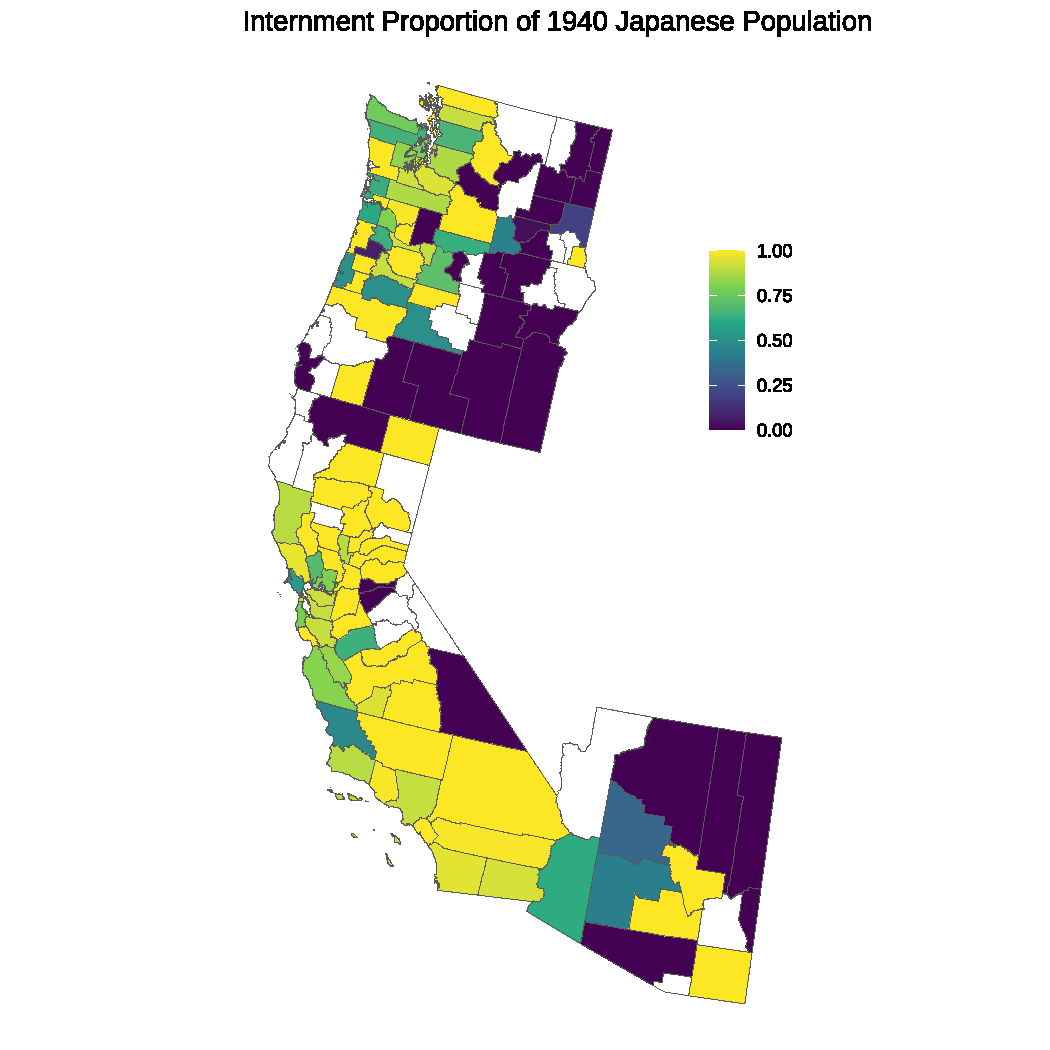
\includegraphics[width=\textwidth]{../figures/pr_interned_map.pdf}
  \end{adjustbox}
  % 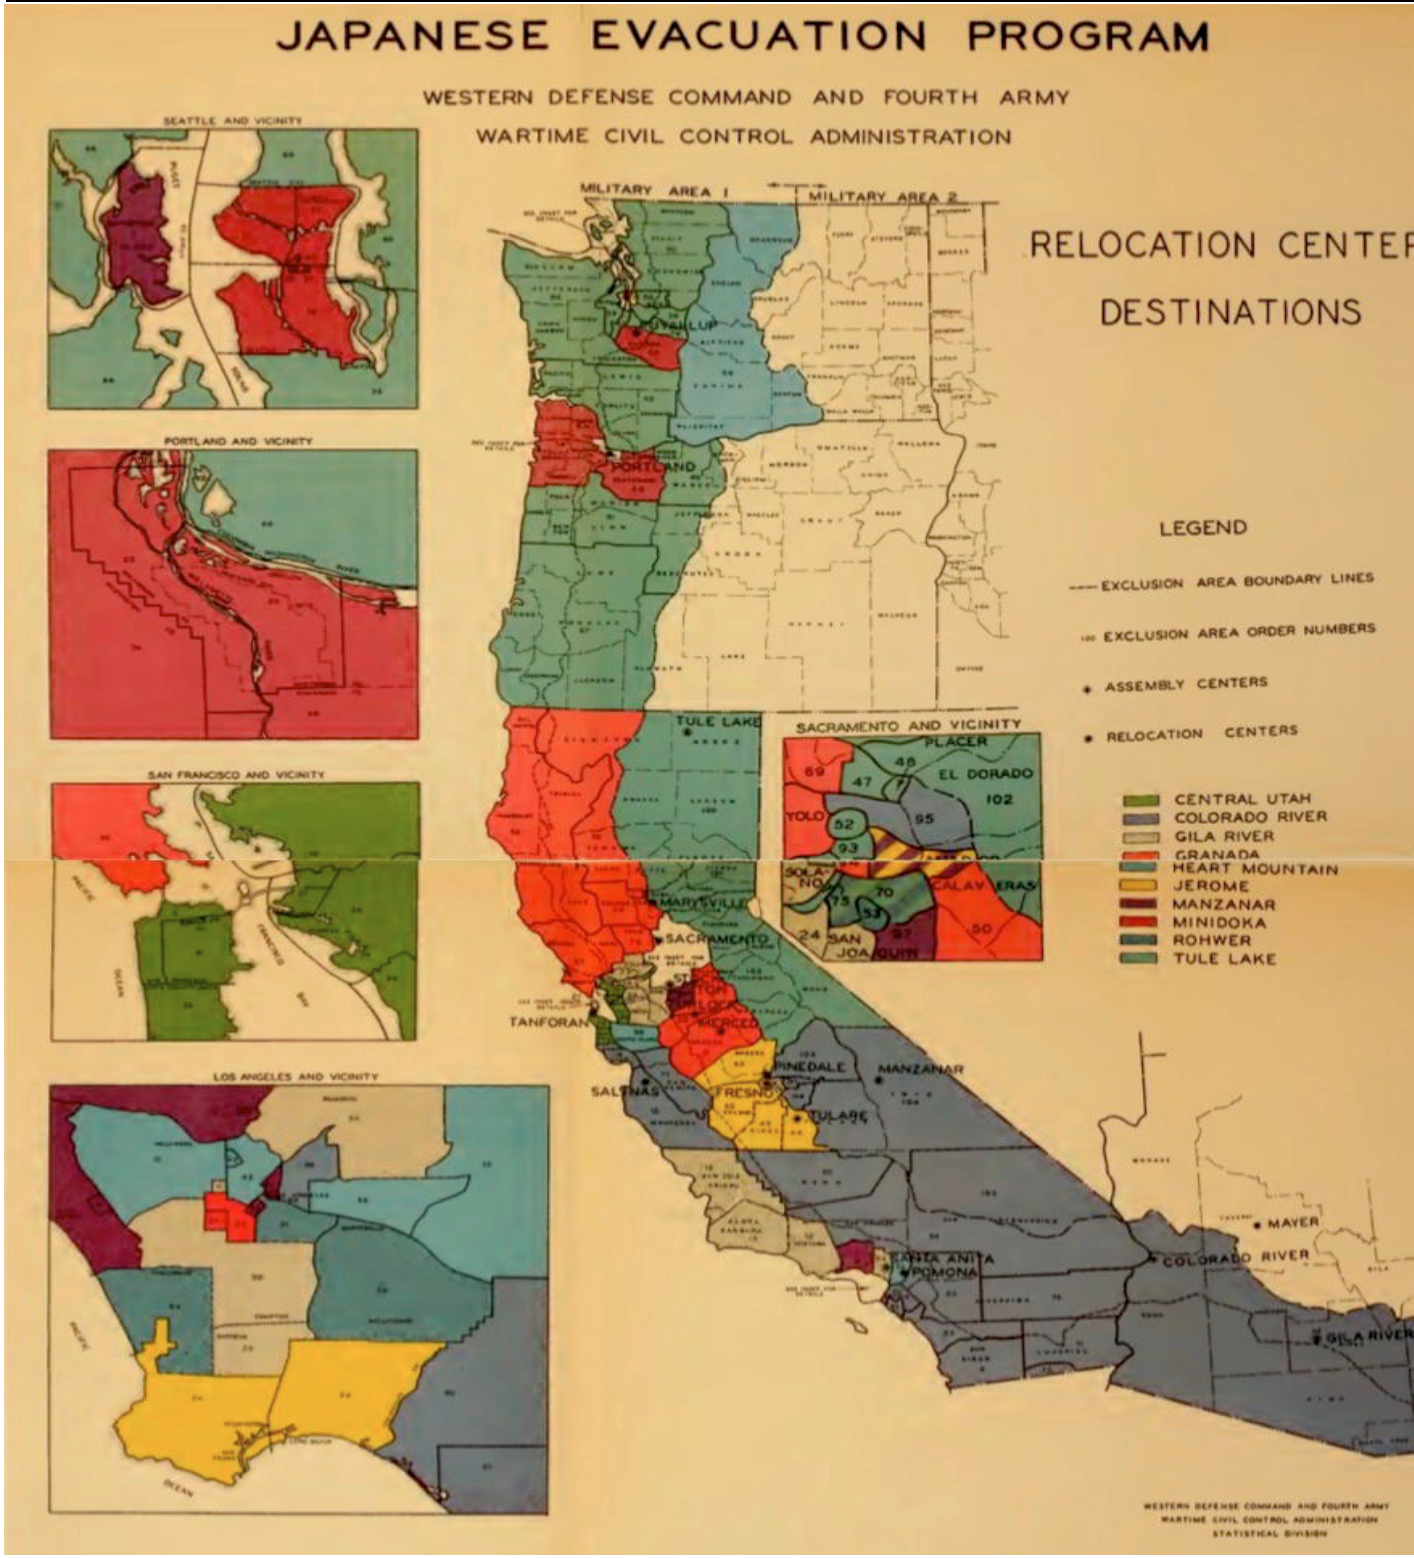
\includegraphics[height=5cm]{../figures/WRAzonesmap.png} \\
  \footnotesize
  Interned proportions are calculated as the number of internees from the county 
  divided by the county's Japanese population in the 1940 full-count census.
  Counties in white had zero Japanese respondents in the 1940 census.
  % The map on the below comes from the 1942 Western Defense Command's Final Report \citep{dewittjohnl.FinalReportJapanese1943}
  % and shows in color the evacuation areas along the West Coast.
\end{figure}
